
\chapter{Grundlagen}
%Harm
\section{Raspberry Pi}\label{Raspberry}
%TODO: Quellen!
Der Raspberry Pi wurde von der britischen Raspberry Pi Foundation entworfen um jungen Menschen den Erwerb von Programmier- und Hardwarekenntnissen zu
ermöglichen. Die Bezeichnung Raspberry Pi folgt der "`Tradition"' Computer nach Früchten zu benennen wie beispielsweise bei "`Apple"'. Das Pi steht für Phyton Interpreter und soll verdeutlichen, dass der Raspberry mit einem Phyton Interpreter ausgeliefert wird. Er ist ein Einplatinencomputer und für wenig Geld verfügbar. Der Raspberry Pi zeichnet sich durch frei programmierbare Schnittstellen aus um beispielsweise Sensoren anzuschließen.(\cite{SWB-435432907}

Mittlerweile gibt es mehrere Modelle:

\begin{itemize} 
\item Pi Zero 
\item Pi Zero W
\item Pi 1 Modell A
\item Pi 1 Modell A+
\item Pi 1 Modell B
\item Pi 1 Modell B+
\item Pi 2 Modell B
\item Pi 3 Modell B 
\end{itemize}

Aufgrund der Vielzahl der mittlerweile verfügbaren Modelle konzentriert sich die genauere Beschreibung auf die Modelle "`2 Modell B"' und "`3 Modell B"':

\begin{table}[h]
\centering
\caption{Vergleich von Raspberry Pi 2 und 3 \cite{CortexA7} \cite{CortexA57}}
\label{tab:VergleichRaspberry}
\begin{tabular}{lll}
Kriterium                    & Raspberry Pi 2        					& Raspberry Pi 3           \\
Veröffentlichungsdatum       & Februar 2015          					& Februar 2016             \\
CPU                          & ARM Cortex-A7   & ARM Cortex-A57           \\
CPU-Geschwindigkeit (in MHz) & 900             & 1200                     \\
CPU-Kerne                    & 4                              & 4                        \\
Arbeitsspeicher (in MB)      & 1024                  					& 1024                     \\
USB 2.0-Anschlüsse           & 4                     					& 4                        \\
Ethernetschnittstelle        & 10/100 MBit Ethernet  					& 10/100 MBit Ethernet     \\
W-Lan                        & \multicolumn{1}{c}{-} 					& 802.11b/g/n (2,4 Ghz)    \\
Bluetooth                    & \multicolumn{1}{c}{-} 					& Bluetooth 4.1 Low Energy \\
Anzahl GPIO-Pins             & 26                    					& 26                      
\end{tabular}
\end{table}
 
Die Modelle Raspberry Pi 2 Modell B und Raspberry Pi 3 Modell B unterscheiden sich nur in wenigen Eigenschaften. Der Raspberry Pi 3 hat eine höher getaktete CPU, WLAN und Bluetooth.

%Jan
\section{Sprachen}

\subsection{Python}\label{Python}
\textsc{Johannes Hubertz}\cite{hubertz2016softwaretests} schreibt, dass Python für alle gängigen Betriebssysteme verfügbar wären und bei Linux-Distributionen würden sie direkt mit ausgeliefert werden. Der Interpreter eigne sich für manuelle Eingaben, die direkt verarbeitet werden. Ebenfalls eigne sich dieser für die Ausführung von Dateien, die Python-Code enthalten. Eine Eigenheit von Python bestehe darin, alles als Objekt zu behandeln. Der Quelltext sei durch die besondere Einrückung mit Leerzeichen, der die wesentliche Ausführung bestimmt, einfach und gut lesbar. \\
Mit der Scriptsprache Python ist es möglich sein, die Sensoren des Raspberry Pi zu implementieren. Ebenso gibt es die Möglichkeit eine Datenbankschnittstelle und eine Schnittstelle für die Kommunikation unter den Raspberry Pi's zu erstellen.

\subsection{Java}\label{Java}
\textsc{Dietemar Abts} stellt in seinem Buch "'Grundkurs JAVA : von den Grundlagen bis zu Datenbank- und Netzanwendungen"' \cite{abts2015grundkurs} Java als eine universelle Programmiersprache für viele Anwendungen in der Industrie auf Client- und Serverseite dar.
Sie wird als Standard für die Entwicklung von Unternehmenssoftware, Webanwendungen, in technischen Systemen und in mobilen Anwendungen verwendet.
Ein besonderes Merkmal von Java sei die Plattformunabhängigkeit, d.h. Java Anwendungen sind ohne Portierung auf nahezu allen Rechnersystemen lauffähig. Java profitiere von den Erfahrungen mit anderen Programmiersprache wie C, C++ und Smalltalk. Wesentliche Konzepte wurden übernommen und fehleranfällige Eigenschaften wären bewusst ausgelassen, damit die Sprache verhältnismäßig robust und einfach sei.\\
Mit der Programmiersprache Java ist es möglich, die Sensoren des Raspberry Pi's zu implementieren. Ebenso können Datenbankschnittstellen und Schnittstellen zur Kommunikation erstellt werden.

\subsection{\ac{SQL}}
Laut \textsc{Edwin Schick}\cite{schicker2017datenbanken} sei \ac{SQL} eine Zugriffsprache für den Endbenutzer. Als Schnittstelle für den Anwender dominieren inzwischen grafische Oberflächen. Für Datenbankprogrammierer habe die Sprache \ac{SQL} an große Bedeutung gewonnen, insbesondere seit der ersten Normierung (SQL1 1987).\ac{SQL} sei die wichtigste Standardsprache für Datenbanken. \\
Die \ac{SQL} Datenbank soll als Speicher für Daten der Raspberry Pi's dienen. Zusätzlich soll die Daten aus der Datenbank lesbar sein.
\subsection{\ac{HTML}}
\textsc{Valentin Plenk}\cite{plenk2017angewandte} schreibt, dass \ac{HTML} eine textbasierte Auszeichnungssprache sei, die von Menschen für Menschen geschriebene Texte strukturiere. Durch den Webbrowser und Gestaltungsvorlagen wie \ac{CSS} wäre die visuelle Darstellung der Texte bestimmt. \ac{HTML} könne strukturierte Dokumente durch verschieden Gliederungsebenen, Absätze und Tabellen erstellen. Zusätzlich biete es Möglichkeiten Hyperlinks, Bilder und andere multimediale Inhalte wiederzugeben. Die Grundlage des World Wide Webs seien \ac{HTML}-Dokumente, die durch die Webbrowser dargestellt werden. \\
Diese Auszeichnungssprache soll zur Darstellung des Projektes im Webbrowser dienen und somit die gesammelten Messdaten u.v.m. anzeigen.

\subsection{\ac{PHP}}
\textsc{Günther Pomaska} schreibt in seinem Buch "'Webseiten-Programmierung Sprachen, Werkzeuge, Entwicklung"' \cite{pomaska2012webseiten-programmierung}, dass \ac{PHP} für die Web-Programmierung entwickelt wurde. Typische Aufgaben von Internetanwendungen wären durch die Sprache abgedeckt, z.B.: Übermittlung von Formulardaten, Anbindung von Datenbanken oder Erzeugen von Webseiten. Gründe für den Einsatz von \ac{PHP} seien, die weite Verbreitung des Open Source-Projekts mit der plattformübergreifenden Anwendung auf unterschiedlichen Betriebssystemen. Der Entwickler profitiere von der Verfügbarkeit von Programmierbausteinen.\\
Mit der Programmiersprache \ac{PHP} sollen die Daten aus der Datenbank ausgelesen und dynamisch geladen werden.

\subsection{JavaScript}
Laut \textsc{Günther Pomaska} \cite{pomaska2012webseiten-programmierung} sei JavaScript nicht mit der objektorientierten Programmiersprache Java in Verbindung zu bringen, obwohl die Syntax der Sprachelemente in vielen Fällen gleich sei. JavaScript ergänze die Funktionalität von Web-Browsern und sei eine objektbasierte Skriptsprache. Der Browser könne den Inhalt einer Webseite nur statisch abbilden, mit Hilfe von JavaScript können Inhalte dynamisch dargestellt werden. Durch Benutzerzugriffe wären Elemente dynamisch veränderbar, ohne die Seite neu laden zu müssen.\\
Mit der Scriptsprache JavaScript sollen die Daten aus der Datenbank dynamisch geladen und dargestellt werden.

%Alex
\section{Sensoren}\label{Sensoren_Planung}
Der Raspberry Pi besitzt mit den \ac{GPIO} Pins eine Möglichkeit Sensoren anzusteuern. Nach der Dokumentation der Raspberry Pi Foundation\cite{GPIOMode77:online} können die \ac{GPIO} Pins 3.3V liefern und digitale Signale annehmen. Das neue Raspberry Pi 3 Modell hat den gleichen Aufbau der \ac{GPIO} Pins und die gleiche Pinbelegung. Schematisch wird die \ac{GPIO} Schnittstelle wie folgt dargestellt.
\begin{figure}[h]
	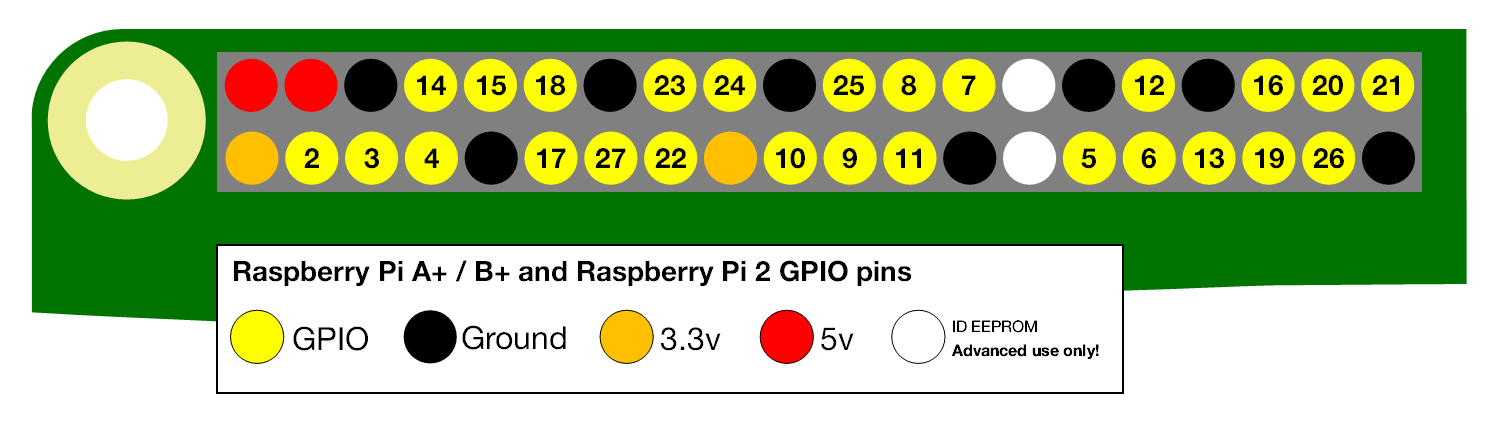
\includegraphics[width=\textwidth]{Bilder/Kapitel2/gpio_pins_pi2.png}
	\caption[Schema GPIO Pins]{Schematische Darstellung der GPIO Pins. Entnommen aus der Raspberry Pi Dokumentation\cite{GPIOMode77:online}.}
	\label{fig:Kapitel2/gpio_pins_pi2.png}
\end{figure}
\noindent
An den vorhandenen 3.3V und 5V Anschlüsse können Sensoren betrieben werden. Dennoch sind nicht alle Sensoren verwendbar. Der Raspberry Pi verfügt nur über die Möglichkeit digitale Signale an den \ac{GPIO} Pins zu verarbeiten. Es werden jedoch neben digitalen auch analoge Sensoren benötigt. Diese können nicht direkt an die Pins angeschlossen werden, aber das Problem wird mit einem \ac{A/D-Wandler} gelöst. \\
Die Erweiterungsplatine RPi-Explorer 700 von Joy-IT \cite{joyitrpi87:online} beinhaltet einen \ac{A/D-Wandler} an dem Analoge Pins angeschlossen werden können. Durch die Erweiterung ist es möglich bis zu vier analoge Sensoren an einem Sensorknoten betrieben werden. \\
Die \ac{GPIO} Schnittstelle unterstützt nur eine maximale Versorgungsspannung von 3.3V, was für die Sensoren ausreichend ist. Durch die Kompatibilität zum Arduino und dem Raspberry Pi können die Sensoren sowohl mit 5V als auch mit 3.3V betrieben werden.
Folgende Sensoren von Allnet\cite{111861pd90:online} werden  im \fullref{Verdrahtung_der_Sensoren} verwendet:
\begin{description}
\item[Temperatur und Luftfeuchtigkeitssensor] \hfill \\
	Der Sensor, KY-015, vom Typ DHT11 kann Temperaturen von 0 bis 50$^\circ$C mit einer Messungenauigkeit von $\pm$ 2$^\circ$C. Die Luftfeuchtigkeit kann im Bereich von 20 bis 95\% ($\pm$ 5\%) gemessen werden. Hierbei handelt es sich um einen digitalen Sensor.  
\item[Flammensensor]\hfill \\
	Der KY-026 besteht aus einer Fotodiode und einem \ac{Poti}. Die Fotodiode kann Wellenlängen im Bereich von etwa 720 - 1100 nm detektieren. Die Diode hat einen Erfassungswinkel von etwa 60$^\circ$. Der \ac{Poti} wird zur Empfindlichkeitseinstellung genutzt, somit kann eine Reichweite von etwa  ein bis sieben Metern abgedeckt werden. Der Sensor besitzt einen "'Digital Out"'-Pin, der high active geschalten wird. Sobald eine Flamme erkannt wird, liegt eine logische 1 auf dem Pin. Der "'Analog Out"'-Pin liefert ein analoges Signal, an welchem bei einer gemessenen Flamme eine niedrige Spannung anliegt.
\item[Lichtschranke]\hfill \\
	Das KY-010 Modul ist eine Lichtschranke, die beim Unterbrechen eine logische 1 an dem digitalen Ausgangspin liefert.
\item[Mikrofon]\hfill \\
	Das Mikrofon, KY-038, hat den gleichen Aufbau wie der Flammensonser. Im Gegensatz zum Flammensensor wird hierbei ein Mikrofonmodul, statt einer Fotodiode genutzt. Die Signale am Digital Out und Analog Out haben die gleiche Funktionalität wie beim Flammensensor. Dieses Modul dient hauptsächlich zur Detektion von kurzen aber lauten Tönen. Ein Anwendungsbeispiel hierfür ist eine Alarmfunktion. Beispielsweise kann das Zerbrechen eines Fensters festgestellt werden.
\item[Lichtsensor]\hfill \\
	Der Lichtsensor KY-018, bestehend aus einem Fotowiderstand, hat bei Dunkelheit einen Widerstand $>$20M$\Omega$ und bei Helligkeit $<$ 80$\Omega$. Damit kann bestimmt werden, ob in einem Zimmer das Licht brennt. Der Lichtsensor liefert ein analoges Signal.
\item[Schocksensor]\hfill \\
	Der Erschütterungssensor liefert eine logische 1 an dem Ausgangspin, falls eine Erschütterung festgestellt wurde. Das dient exemplarisch zur Umsetzung einer Schritterkennung am Boden.
\end{description}

%Harm
\section{WLAN}
\subsection{Standard}
%TODO: "Ich will mehr, viel mehr" - Rammstein
Die Vernetzung erfolgt über ein Funknetz nach dem WLAN-Standard 802.11n. 

\subsection{Verschlüsselung}
%TODO: Einleitung
Da WLAN die Luft als Übertragungsmedium verwendet und jeder darauf zugreifen kann, verdient die Verschlüsselung des Datenverkehrs besondere Aufmerksamkeit. Die Verschlüsselung verhindert, dass dritte die Kommunikation des Endgeräts mit dem Access-Point mitlesen können. Verschlüsselung hat allerdings das Problem, dass beide Geräte ein Geheimnis teilen müssen. Dieses Geheimnis wird Schlüssel genannt. Es gibt aktuell drei Verschlüsselungsverfahren, die verwendet werden können. \ac{WEP} und \ac{WPA} sind aber bereits geknackt und somit nicht mehr sicher.

\subsubsection{\ac{WEP}}
Bei der Standardisierung des Standards 802.11b, 802.11g und 802.11a wurde \ac{WEP} integriert. \ac{WEP} basiert auf einem Stream Ciphering-Algorithmus, bei dem die Daten mit einer Ciphersquenz verschlüsselt werden. Die Sequenz wird mit einem \ac{IV} und einem Schlüssel berechnet. Der \ac{IV} ändert sich für jedes Frame und erzeugt somit wechselnde Ciphering Keys. Der daraus berechnete Schlüssel wird mit den Daten der Nachricht verodert. (vgl. \cite{SWB-430171331})


\begin{figure} [htb]
\begin{centering}
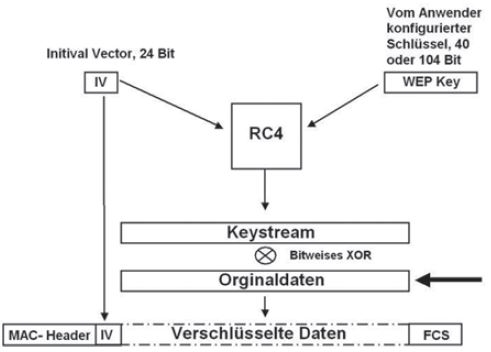
\includegraphics{Bilder/wep_funktionsweise.jpg}
\caption[WEP-Verschlüsselung]{WEP-Verschlüsselung \cite{SWB-430171331}}
\label{wep_funktionsweise}
\end{centering}
\end{figure}

Problematisch an diesem Verfahren ist, dass der Schlüssel bei jedem Teilnehmer eingetragen werden muss und somit nicht Geheim gehalten werden kann. Schwerwiegender ist allerdings, dass jedes verschlüsselte Frame am Anfang die gleiche Bytefolge des \ac{LLC}-Headers beinhaltet. Bestimmte \ac{IV}s werden im Klartext übertragen wodurch ein Angreifer nach 5-6 Millionen Paketen den Schlüssel berechnen kann. Mittlerweile sind auch Anwendungen verfügbar, die selbst Datenpakete erzeugen und so in sehr kurzer Zeit, den Schlüssel berechnen können.(vgl. \cite{SWB-430171331})
%TODO: Kann bei Seitenbedarf noch ausgebaut werden

\subsubsection{\ac{WPA}} 
%TODO: Schluessel in PPE-Schluessel muss geändert werden. Mal mit Alex sprechen warum das ü nicht gefressen wird
Da \ac{WEP} die beschriebenen Schwächen hat ist 802.11i von der \ac{IEEE} entwickelt worden. Da \ac{WPA2} aber \ac{CCMP} voraussetzt, was mehr Leistung benötigt, wurde durch die Industrie \ac{WPA} entwickelt. \ac{WPA} funktioniert auch auf schwächerer Hardware. Als Verschlüsselungsmethode wird \ac{TKIP} und Optional \ac{CCMP} verwendet. Beschrieben wird hier die Funktionsweise mit \ac{TKIP}. \\
\ac{TKIP} verwendet wie \ac{WEP} den RC4-Algorithmus zur Verschlüsselung der Daten aber der Umgang mit Daten und Schlüsseln ist komplexer. \\
Nach \textsc{Klaus Schmeh} \cite{SWB-378541420} ist die Grundlage von \ac{TKIP} der \ac{PMK}, der beiden Seiten bekannt sein muss. Er hat eine Länge von 256 Bit und wird nur zur Ableitung anderer Schlüssel verwendet. Aus einem \ac{IV}, der MAC-Adresse und dem Daten-Schlüssel wird ein \ac{PPE-Schluessel} gebildet. Der \ac{PPE-Schluessel} ist 128 Bit lang und wird für jedes Datenpaket neu generiert.
Der \ac{IV} teilt sich in zwei Teile von denen der erste 16 Bit und der zweite 32 Bit lang ist. Dies ergibt eine Länge von 48 Bit was bereits mehr ist als der 24 Bit \ac{IV} von WEP. Der erste Teil erhöht sich von Paket zu Paket um 1.\\
Der MICHAEL-Schlüssel und die unverschlüsselten Daten werden an die schlüsselabhängige Hashfunktion MICHAEL übergeben, die einen Hashwert berechnet. Die Daten und der Hashwert werden zusammengefügt und es wird mit CRC ein zweiter Hashwert generiert. Verschlüsselt werden die Daten mit beiden Hashwerten nun mit dem RC4-Verfahren und dem jeweils gültigen \ac{PPE-Schluessel}. (vgl. \cite{SWB-378541420})

\begin{figure} [htb]
\begin{centering}
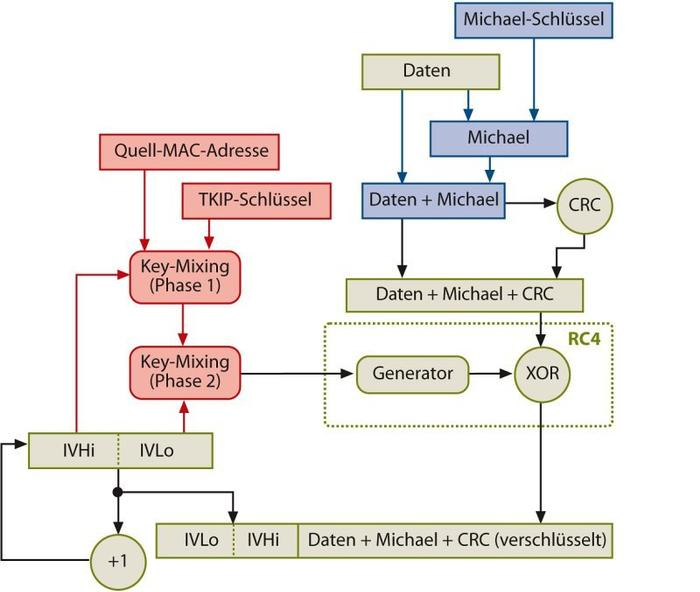
\includegraphics[scale=0.6]{Bilder/wpa_funktionsweise.jpg}
\caption[WPA-Verschlüsselung]{WPA-Verschlüsselung \cite{Heise-WLAN}}
\label{wpa_funktionsweise}
\end{centering}
\end{figure}

\subsubsection{\ac{WPA2}}

Der Vorteil gegenüber \ac{TKIP} ist, dass \ac{CCMP} auf dem \ac{AES}-Verschlüsselungsstandard basiert. Bei \ac{CCMP} wird ein 128 Bit Schlüssel mit 48 Bit Initialisierungsvektor verwendet. \cite{Tanenbaum}
%%


